\documentclass[a4paper,12pt]{report}
\usepackage[utf8]{inputenc}
\usepackage{authblk}
\usepackage{graphicx}
\usepackage{color}

\usepackage{fancyhdr}
\usepackage{titling}
\usepackage{geometry}


\title{\textbf{International Trade process : Letter of Credit (LC) Management using Blockchain technology}}
\author{
\bf Md Sadek Ferdous\\
Brac University\\
sadek.ferdous@bracu.ac.bd\\
\and
\bf Asif Idris Tuhin\\
Shahjalal University of Science and Technology\\
tuhin123000@gmail.com\\
\and
\bf Zahid Khandaker Sumon\\
Shahjalal University of Science and Technology\\
zksumon2017@gmail.com\\
}

\date{October 2021}

\predate{\centering}
\postdate{\vfill\hfill\emph{This report is prepared and submitted by: \textbf{Asif Idris Tuhin - 2017331101}}\hfill}
\usepackage{lipsum}
\pagestyle{plain}


\begin{document}


\maketitle

\pagenumbering{roman}

\section*{Abstract}
Traditional trade processes suffer from a great number of issues about intermediaries, information latency and trust, which, in turn, hinder overall process efficiency.But still there are lack of proper tools for mitigating this problem. The objective of this report is to represent our endeavor of developing a Letter of Credit (LC) Management project using Blockchain technology. This report also represents the using technique of this Lc management project. We have developed this project on the basis of Hyperledger Fabric 2.2.1 . Importer and exporter can deal and run their business safely as well as easily by using this software.


\vspace{100pt}
\section*{Keywords}
Blockchain; Letter of Credit; Trade Finance; Hyperledger Fabric.

\newpage




\tableofcontents



\vspace{100pt}

\begin{table}[h]
    \centering
    \begin{tabular}{|c|c|}
    \hline
         &\textbf{Date}  \\
         \hline
    \textbf{Starting}     & 19 Aug 2020\\
    \hline
    \textbf{Study fundamental Books} & 19 Aug 2020 - 26 Aug 2020\\
    \hline
    \textbf{Time for Selecting Projects} & 16 Sept 2020 - 4 Oct 2020\\
    \hline
    \textbf{First Individual meeting} & 31 Oct 2020\\
    \hline
    \textbf{ First Hyperledger Fabric session} & 6 Nov 2020\\
    \hline
    \textbf{Second Hyperledger Fabric session} & 2 Dec 2020\\
    \hline
    \textbf{Second Individual meeting} & 30 Dec 2020\\
    \hline
    \textbf{Subtask 1} & 30 Dec 2020 - 14 Feb 2021\\
    \hline
    \textbf{Third Individual meeting} & 20 Feb 2021\\
    \hline
    \textbf{Subtask 2} & 20 Feb 2021 - 19 Mar 2021 \\
    \hline
    \textbf{First Submission} & 13 Apr 2021 \\
    \hline
    \textbf{Final Submission} & 25 Apr 2021 \\
    \hline
    \textbf{Viva and Presentation} & 7 May 2021 \\
    \hline
    
    \end{tabular}
    \caption{Project Timeline}
    \label{tab:timeline}
\end{table}


\newpage

\pagenumbering{arabic}

\chapter{Introduction}

\section{Motivation}
International trade allows countries to expand their markets and access goods and services that otherwise may not have been available domestically. But, due to the nature of international dealings, including factors such as distance, differing laws in each country and difficulty in knowing each party personally, International trade become risky. So the use if letters of credit(LC) has become a very important aspect of international trade.

\vspace{15pt}
\section{Defining LC}
A letter of credit is a letter from a bank guaranteeing that a buyer's payment to a seller will be received on time and for the correct amount. So, it becomes indispensable for international transactions since they ensure that payment will be received. Using documentary letters of credit allows the seller to significantly reduce the risk of non-payment for delivered goods, by replacing the risk of the buyer with that of the banks.

\vspace{15pt}
\section{Novelty of this project}
Some analyses and feasibility studies has been conducted to identify and validate the enhancing overall trade performance by blockchain-based international trade process from a perspective of letter of credit \cite{justexploring2019}. Another work has done regarding a potential paradigm shift in trade finance utilizing blockchain technology \cite{chang2020blockchain}. But, still there are lack of such implementation of letter of credit management software using blockchain technology by which importer and exporter can run their business without difficulty. On the other hand, some of the alternative to the Letter of Credit for international trade like Purchase Order Financing has some cons such as While most suppliers would like to be paid by wire transfer, unless your supplier is a fortune 500 company, po finance companies will only pay them using a letter of credit. The do this because a letter of credit ensures that the supplier will only be paid if and when they deliver the goods and more on \cite{purchaseorder2021effects}. So Letter of Credit management using blockchain is very important in this new global Era and We have implemented this project.

\vspace{15pt}
\section{Short Overview of the project}
We have used Hyperledger Fabric 2.2.1 for implementing this project \cite{fabric}. We need Linux operating system(Ubuntu), Docker, Docker Compose, Node js (LTS), cloud database etc. technologies for it. The users who will use this need some of this technologies also.\\
There are four organizations - org1(Buyers), org2(Sellers), org3(Buyer Bank),  org4(Seller Bank), {\large Shown in figure \ref{fig:organization}}. Fabric 2.2.1 test network only makes 2/3 orgs. So, we edited the test network scripts for creating 5 orgs. In this project, it is possible to create many seller and buyer member through sign up. But, for the simplicity, we have restricted only one Seller Bank and one Buyer Bank.
\begin{figure}[h]
    \centering
    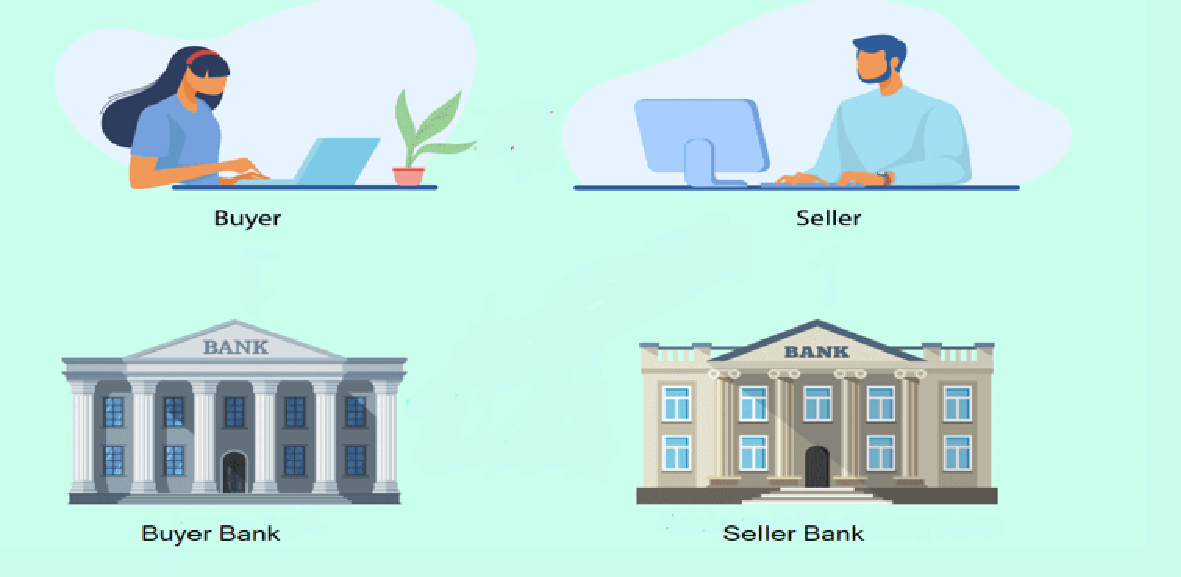
\includegraphics[width=0.75\textwidth]{Organization.pdf}
    \caption{Four Organizations}
    \label{fig:organization}
\end{figure}


\chapter{Problem Definition}
Letters of credit have become a crucial aspect of international trade , due to the difficulty of knowing each party personally. Using LC allows the seller to significantly reduce the risk of non-payment for delivered goods, by replacing the risk of the buyer with that of the banks.

Blockchain resolves this problem. Using blockchain technology can help streamline the manual processing of import/export documentation, improve security by reducing errors, make companies' working capital more predictable and increase convenience for all parties through mobile interaction. So application of Blockchain to Letter of Credit is very important and it has been done in our project. 

\chapter{Background}
\section{How LC works}
A letter of credit, or ``credit letter" is a letter from a bank guaranteeing that a buyer's payment to a seller will be received on time and for the correct amount. In the event that the buyer is unable to make a payment on the purchase, the bank will be required to cover the full or remaining amount of the purchase.\\
 Figure \ref{fig:lcprocess} shows the process of LC. Here, $Importer=buyer$, $Issuing Bank=Buyer's Bank$, $Exporter=Seller$ and $Advising Bank= seller's Bank$.

\begin{figure}[h]
    \centering
    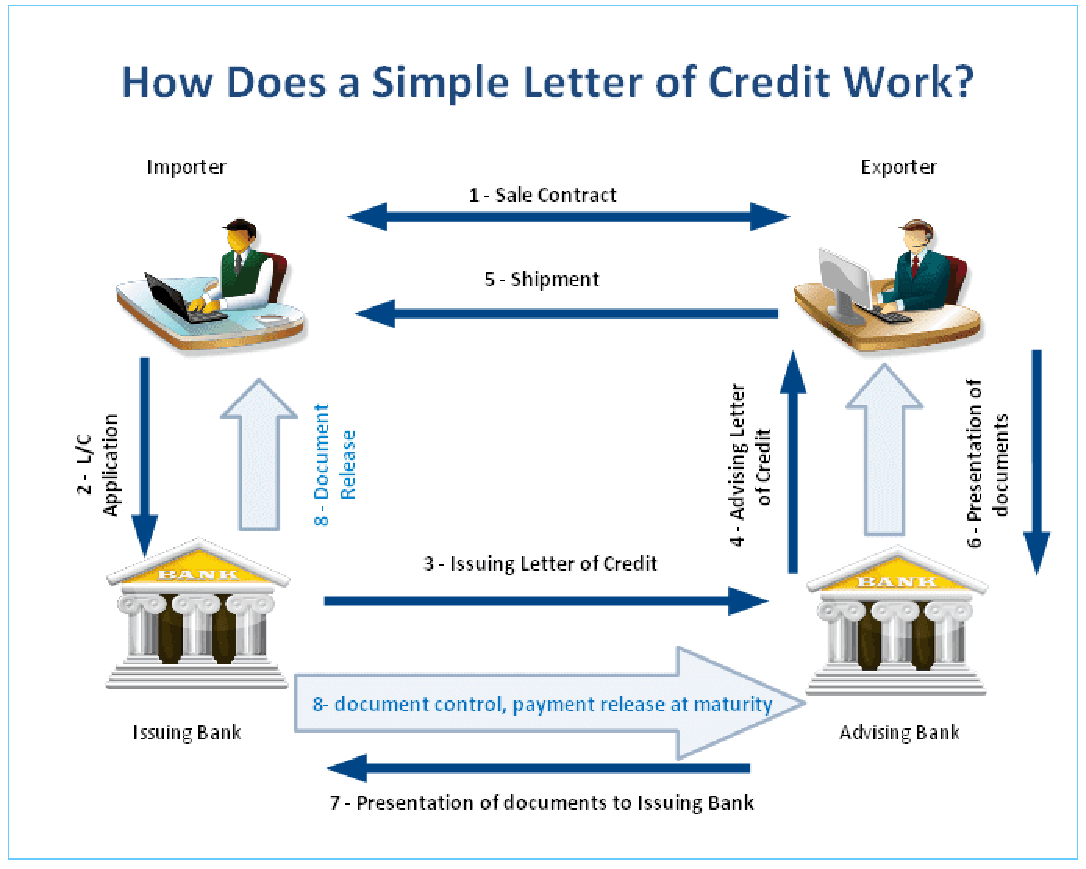
\includegraphics[width=0.7\textwidth]{letter-of-credit-process.pdf}
    \caption{LC Process}
    \label{fig:lcprocess}
\end{figure}

\section{Important Terms}
Here are some related and important term that we should know before dive into the project.
\subsection{Blockchain}
Blockchain is a shared, immutable ledger that facilitates the process of recording transactions and tracking assets in a business network. An asset can be tangible (a house, car, cash, land) or intangible (intellectual property, patents, copyrights, branding). Virtually anything of value can be tracked and traded on a blockchain network, reducing risk and cutting costs for all involved\cite{Blockchain}.
\subsection{Hyperledger Fabric}
Hyperledger Fabric is intended as a foundation for developing applications or solutions with a modular architecture. Hyperledger Fabric allows components, such as consensus and membership services, to be plug-and-play. Its modular and versatile design satisfies a broad range of industry use cases. It offers a unique approach to consensus that enables performance at scale while preserving privacy\cite{fabric1}.
\subsection{Node.js}
As an asynchronous event-driven JavaScript runtime, Node.js is designed to build scalable network applications. In the following, Figure \ref{fig:node} ``Hello World" example,many connections can be handled concurrently. Upon each connection, the callback is fired, but if there is no work to be done, Node.Js will sleep.

\begin{figure}[h]
    \centering
    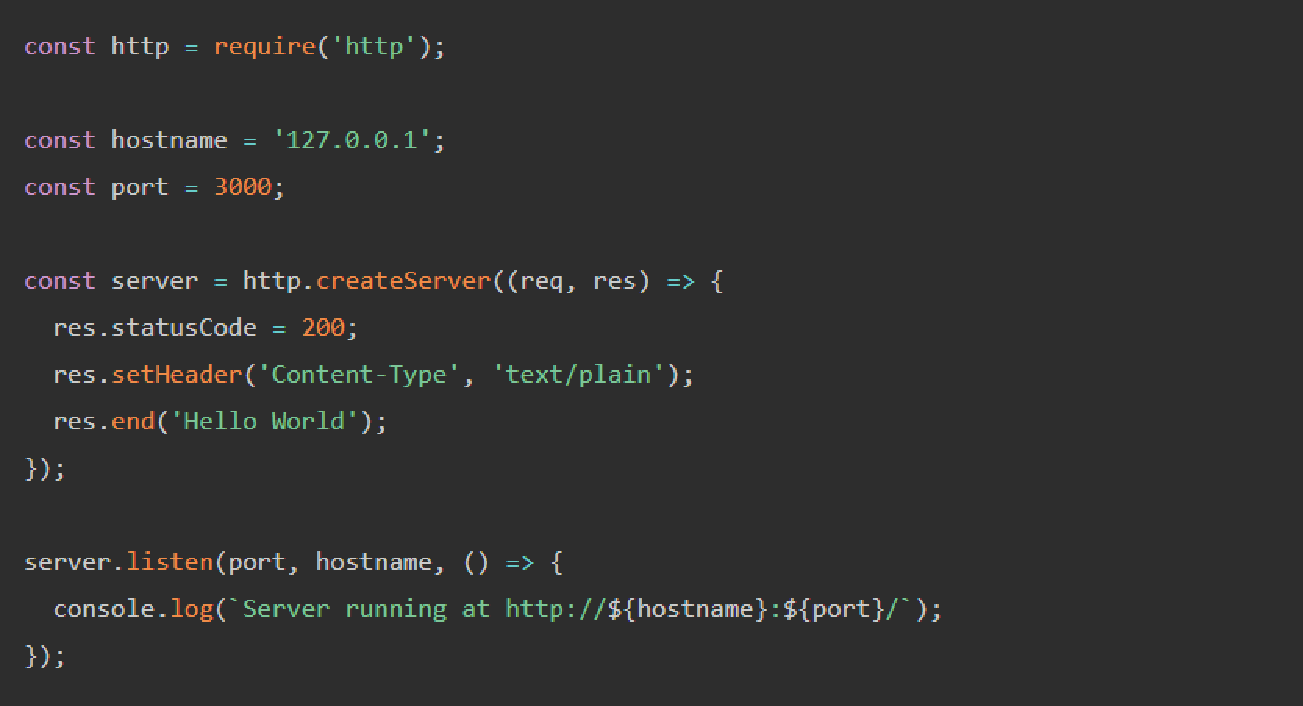
\includegraphics[width=0.7\textwidth]{nodejs.pdf}
    \caption{Hello World in node.js}
    \label{fig:node}
\end{figure}
\subsection{Utility Server}
The Utility Server is a virtual machine that can optionally be connected to your RelativityOne instance. It contains additional support tools to help you work with data in your RelativityOne staging area before editing and loading it into your RelativityOne instance. You access your Utility server through a remote desktop connection, using an issued set of credentials and a custom IP address.\\
Once you are connected to your Utility Server, you can perform the following actions:

\begin{itemize}
    \item \textbf{Access a mapped drive for the file share }(TenantUser accounts) - access your uploaded files to edit in the staging area before you add them to your RelativityOne workspaces or save them to a RelativityOne file storage location. You can also access and verify any production sets before you download them locally.
    \item \textbf{Install applications} - if you have TenantAdmin access you can install applications.
    \item \textbf{Manage user administration} - if you have TenantAdmin access and have Terminal Services licensed on the computer you can manage user administration yourself.
\end{itemize}

\subsection{Cloud Database}
A ``cloud database" can be one of two distinct things: a traditional or NoSQL database installed and running on a cloud virtual machine (be it public cloud, private cloud, or hybrid cloud platforms), or a cloud provider’s fully managed database-as-a-service (DBaaS) offering. The former, running your own self-managed database in a cloud environment, is really no different from operating a traditional database. Cloud DBaaS, on the other hand, is the natural database equivalent of software-as-a-service (SaaS): pay as you go, and only for what you use, and let the system handle all the details of provisioning and scaling to meet demand, while maintaining consistently high performance\cite{cloud}.

\chapter{Main Methodology}
\section{Architectural overview}
{\large As we can see Figure \ref{fig:archi}}, the 4 organizations create channel and install chaincode. Frist two node.js servers can have many users. Though Buyers\&Sellers organizations are like a centralized entity, they can never get the users hex secret string which is used for creating private-public key pair. Users' hex secret string never goes through the 4 organizations node.js servers. All users use an utility server for sending all payload(Lc details) and secret hex string and getting public key string and sign.\\
In real world situations, Users just have to prove that they are the real owner of the public keys mentioned in the ledger and that's very easy.


\begin{figure}[h]
    \centering
    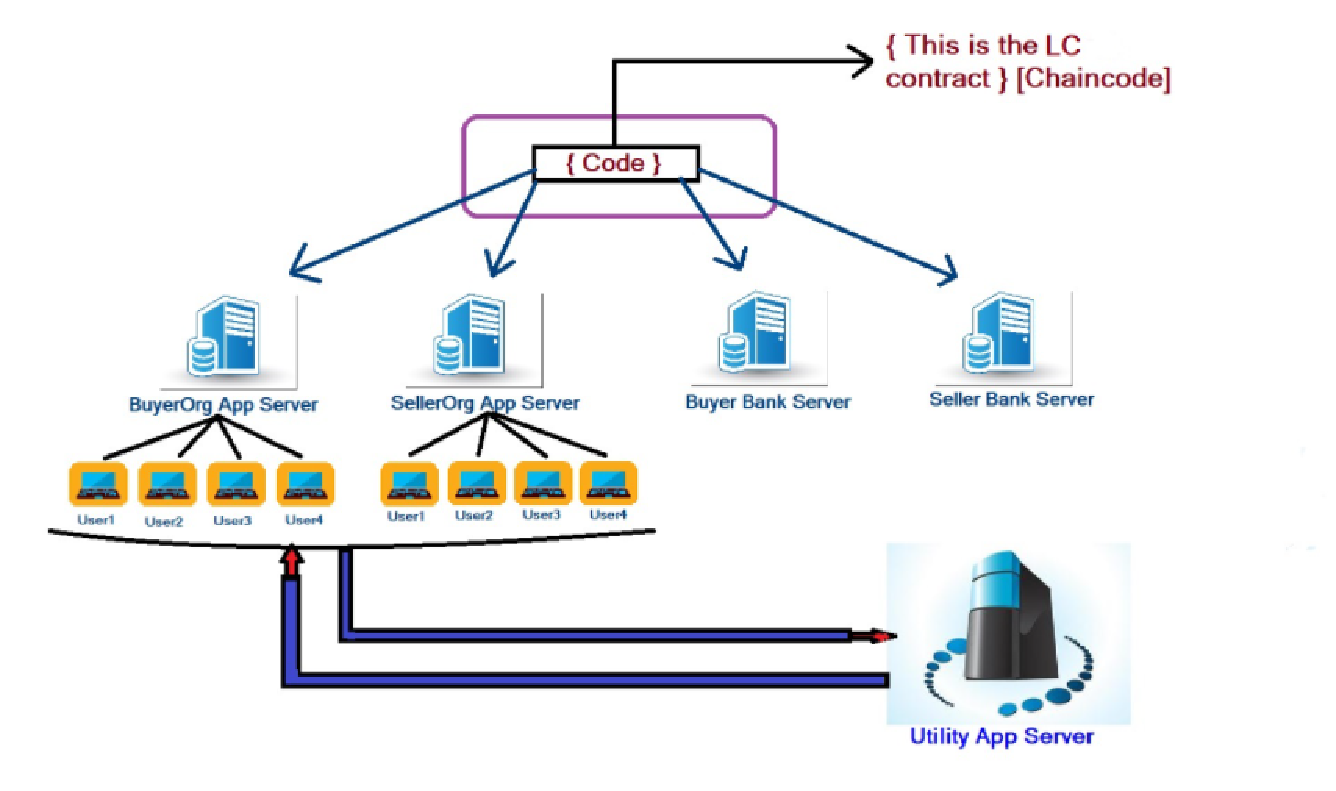
\includegraphics[width=0.81\textwidth]{Archi.pdf}
    \caption{Architectural view}
    \label{fig:archi}
\end{figure}

\section{Chaincode API Access control}
We made all of the 4 node.js servers. There isn't any function in them which should not be their. Example : seller should not be able to invoke buyers bank verify function. Even if we implement this kind of function in server it will get rejected on the chaincode. Because we are checking the fabric MSP ID in all functions. If there is a contradiction the functions will immediately return without heading further.
\vspace{10pt}
\section{NoSql Cloud Database}
All servers (except the utility) are connected to their own MongoDB cloud databases. So, when testing there should be internet connection. We gave all server secrets, email service secrets and MongoDB uri in .env files, So it will work fine.
\vspace{10pt}
\section{Hashing Algorithm}
For all the signing and sign verification, we use node js elliptic library. We are using elliptic's EDDSA algorithm\cite{eddsa}. For the curve selection, we have used ed25519\cite{eddsa} which is considered to be a very secure curve. On lc, we are giving unique lc id based on product details string hash's first 8 characters. This hash is done by crypto library's md5 hashing\cite{md5}. For password hashing and verifying, we have used bcrypt library.
\vspace{10pt}
\section{System Notification flow}
When Buyersbank or Sellersbank does something, it notifies all other 3 servers and the servers save them in cloud database.\\
When seller makes an LC, it notifies Buyers organization (all saved in cloud).\\
When buyer approves an LC, it notifies Buyers Bank (all saved in cloud).

\vspace{30pt}
{\color{magenta}Note :} All account related information (not secret hex string ) like
notification list, account, email, password (hashed with bcrypt library) is
stored on MongoDB Cloud Database, Our login session is managed by
jsonwebtoken and browser cookies (1h expire time). 

\chapter{Features}
\section{How to Run it}
We need to install pm2 module globally in node js as bellow:
\begin{figure}[h]
    \centering
    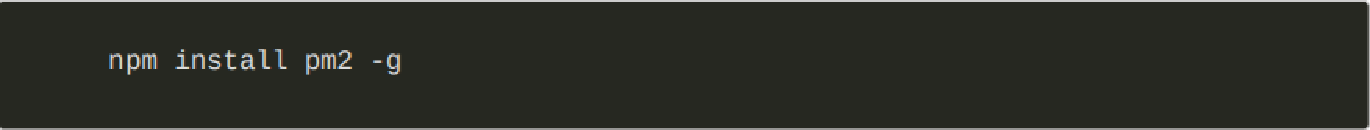
\includegraphics[width=0.7\paperwidth]{npm.pdf}
    \caption{npm install}
    \label{fig:npm}
\end{figure}


Now, clone our github repo in the same directory where your fabric-samples folder is located. \begin{figure}[h]
    \centering
    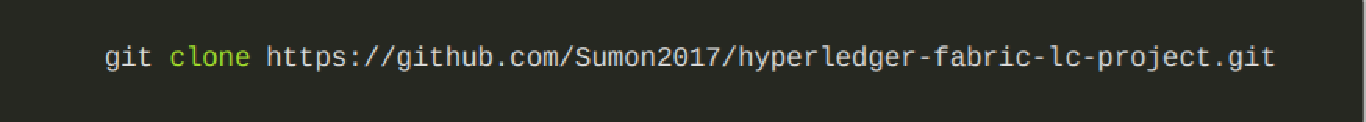
\includegraphics[width=0.7\paperwidth]{gitCapture.pdf}
    \caption{git repo}
    \label{fig:gitrepo}
\end{figure}

\newpage

\textbf{Note:} hyperledger-fabric-lc-project and fabric-samples should be on same directory. (see the fig:\ref{fig:directory})

\begin{figure}[h]
    \centering
    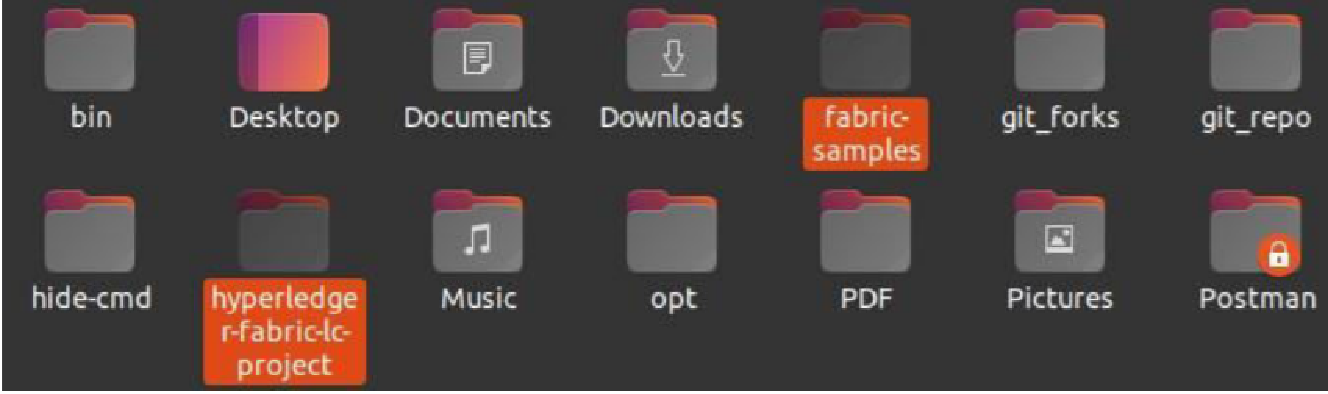
\includegraphics[width=0.8\textwidth]{directoryCapture.pdf}
    \caption{Directory}
    \label{fig:directory}
\end{figure}

Open up a terminal in \textbf{hyperledger-fabric-lc-project/onoff} \\
Now, from \textbf{onoff} directory give excecute permission to our scripts.(see in fig \ref{fig:chmod})

\begin{figure}[h]
    \centering
    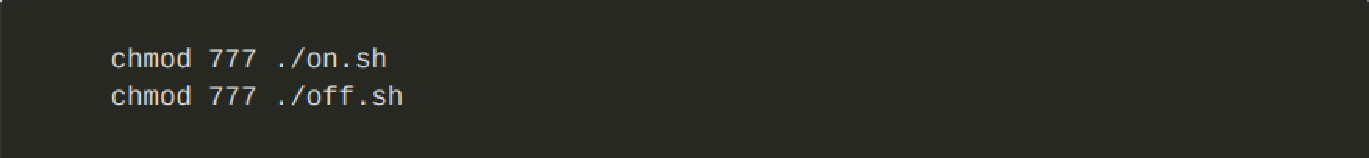
\includegraphics[width=0.7\paperwidth]{chmodCapture.pdf}
    \caption{Giving Executive permission}
    \label{fig:chmod}
\end{figure}


Now from \textbf{onoff} directory to satrt the program run :
\begin{figure}[h]
    \centering
    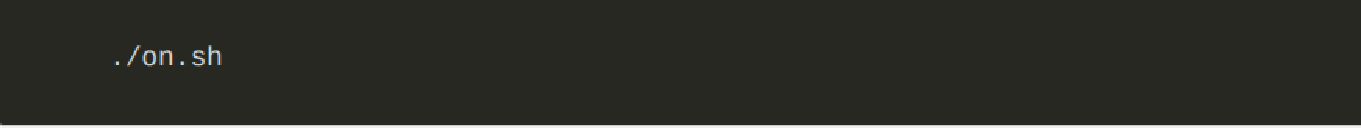
\includegraphics[width=0.7\paperwidth]{onCapture.pdf}
    \caption{Starting the program}
    \label{fig:on}
\end{figure}
\\\textbf{Cautious:} you have to be in \textbf{onoff} directory.\\


\vspace{5pt} 
This takes between 10-15 minutes depending on your hardware and internet speed. It create the fabric network (creating channel, installing chaincode) and 5 node.js servers (we can see them by [docker ps -a] and [pm2 list] ).\\

\newpage
To stop it, run : 
\begin{figure}[h]
    \centering
    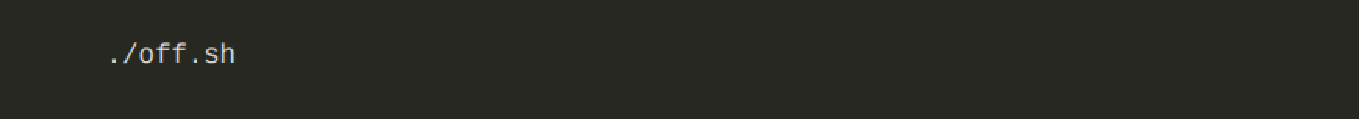
\includegraphics[width=0.7\paperwidth]{offCapture.pdf}
    \caption{Stopping the program}
    \label{fig:off}
\end{figure}
\\\textbf{Cautious:} you have to be in \textbf{onoff} directory.\\
At the end of it, success will be printed.\\
Now Open browser and make 4 new tabs on the browser and hit the following links:\\
\textbf{localhost:3001/index.html}\\
\textbf{localhost:3002/index.html}\\
\textbf{localhost:3003/index.html}\\
\textbf{localhost:3004/index.html}\\
These are BuyersOrgApp, SellersOrgApp, BuyersBank and SellersBank accordingly.

\vspace{20pt}
We find some crypto materials in this project but these will get overriten with new valid crypto materials. 

\section{User Manual}
\begin{itemize}
\item {\color{cyan}Step 1:} Sign up in sellersorgapp and buyersorgapp. We get our verification code in your email. If we don't find it, check spam folder. Then verify with it. (if we don't want to do this, we will give two premade accounts for login.)
\item {\color{cyan}Step 2:}  Login for sellersorgapp and buyersorgapp.
\item {\color{cyan}Step 3:} From sellers organization app create an LC and get pub\_key and sign (with hex string secret).
\item {\color{cyan}Step 4:} create LC from sellers organization app.
\item {\color{cyan}Step 5:} From buyers organization app check notifications for the LC id and approve with our individual specific sign.
\item {\color{cyan}Step 6:} From buyersbank check notifications and issue the LC.
\item {\color{cyan}Step 7:} From sellersbank check notifications and send shipment details. (This should be a string.)
\item {\color{cyan}Step 8:}  From buyersbank check notifications and send transaction money payment details. (This should also be a string). This is the last step and all is done.

\end{itemize}


{\color{green}Tips :} Use dummy strings in shipment details and transaction details for testing purpose. You can also corrupt sign by changing data(after getting pub\_key and sign in step 3) and see if buyer/buyers bank takes it.



\section{Premade account}

Table \ref{tab:premade} showing premade accounts for seller or buyer.

\begin{table}[h]
    \centering
    \begin{tabular}{|c|c|}
    \hline
    \textbf{Sellers Org App}     &\textbf{Buyers Org App}  \\
    \hline
    Username : sumon     & Username : tuhin\\
    \hline
    \texttt{zksumon2017@disbox.org} & \texttt{tuhin123@disbox.org} \\
    \hline
    Password : 1234 & Password : 1234\\
    \hline
    \end{tabular}
    \caption{Premade Account for seller and buyer}
    \label{tab:premade}
\end{table}


\section{Running from different Organization}

Figures - \ref{fig:2}, \ref{fig:1}, \ref{fig:5}, \ref{fig:7}, \ref{fig:8} is given bellow demonstrating some situations when we run from different organization :

\vspace{20pt}

\begin{figure}[h]
    \centering
    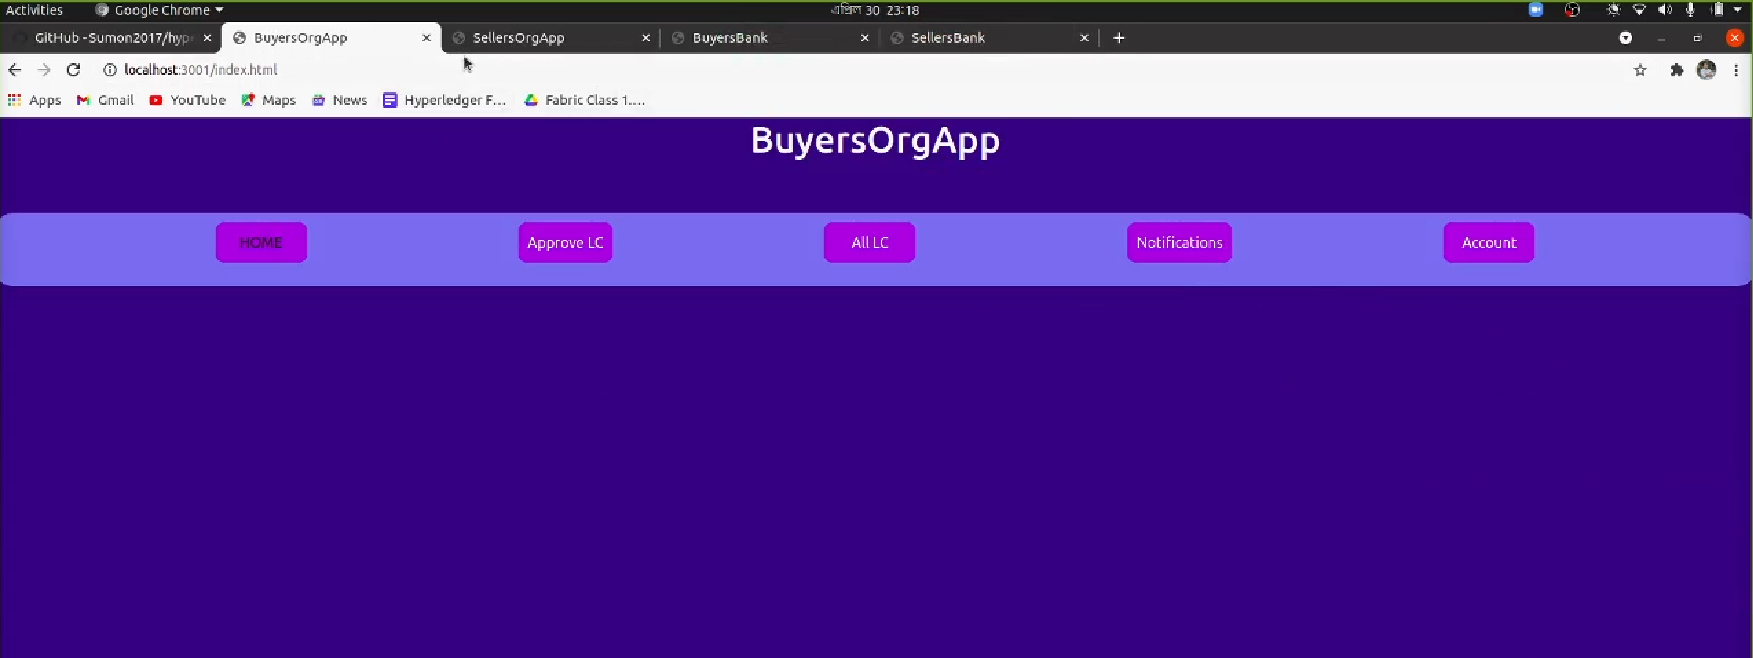
\includegraphics[width=0.7\paperwidth]{2.pdf}
    \caption{Buyer Organization}
    \label{fig:2}
\end{figure}

\begin{figure}[b]
    \centering
    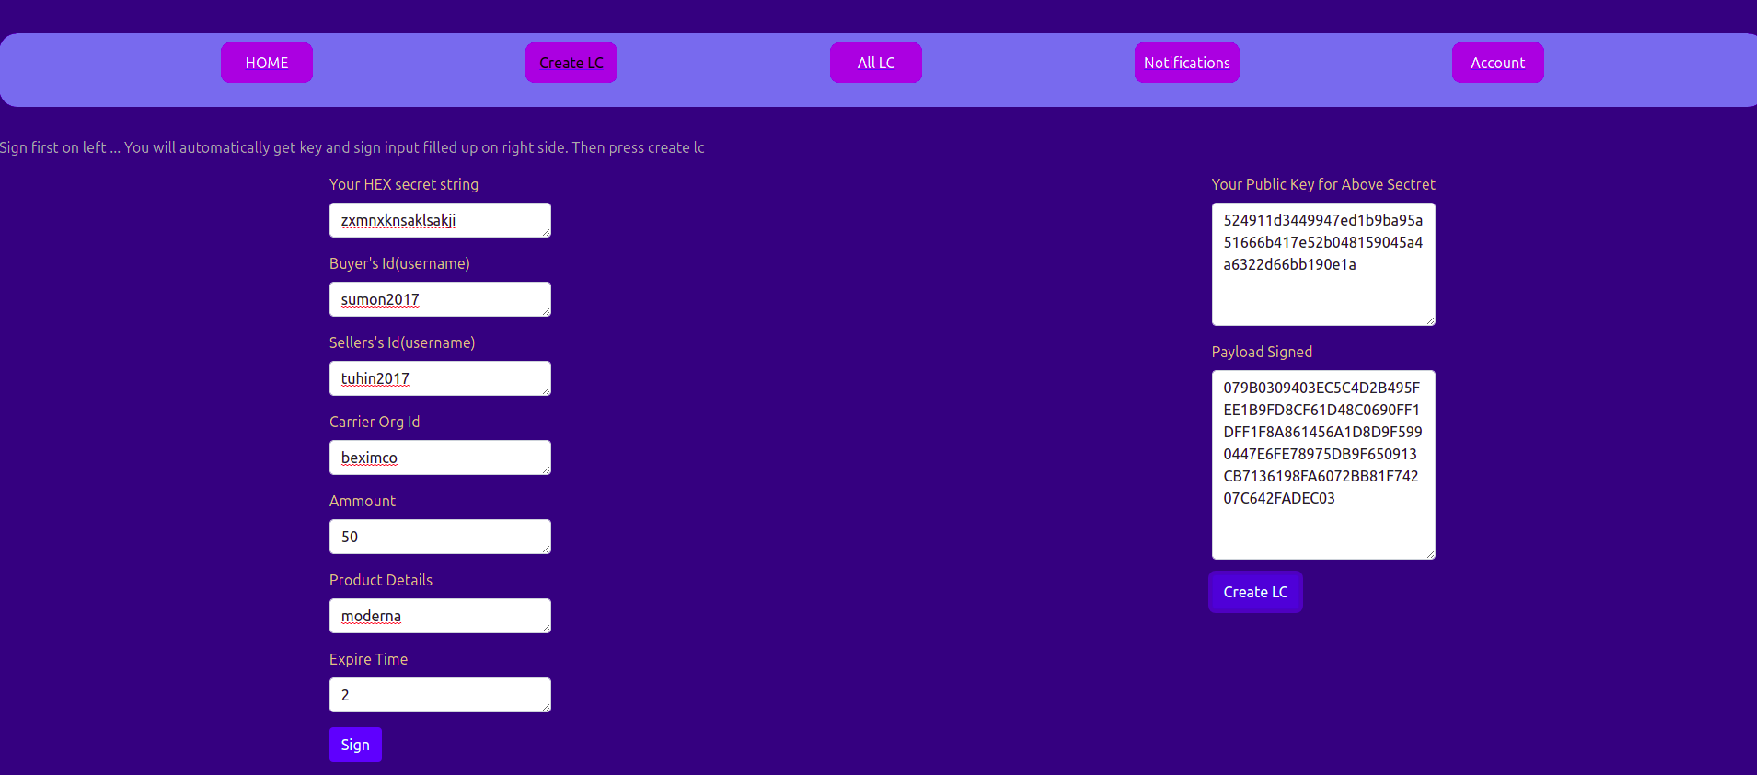
\includegraphics[width=0.7\paperwidth]{1 (1).pdf}
    \caption{Buyer signing with product,time,seller details}
    \label{fig:1}
\end{figure}


\newpage

\begin{figure}[h]
    \centering
    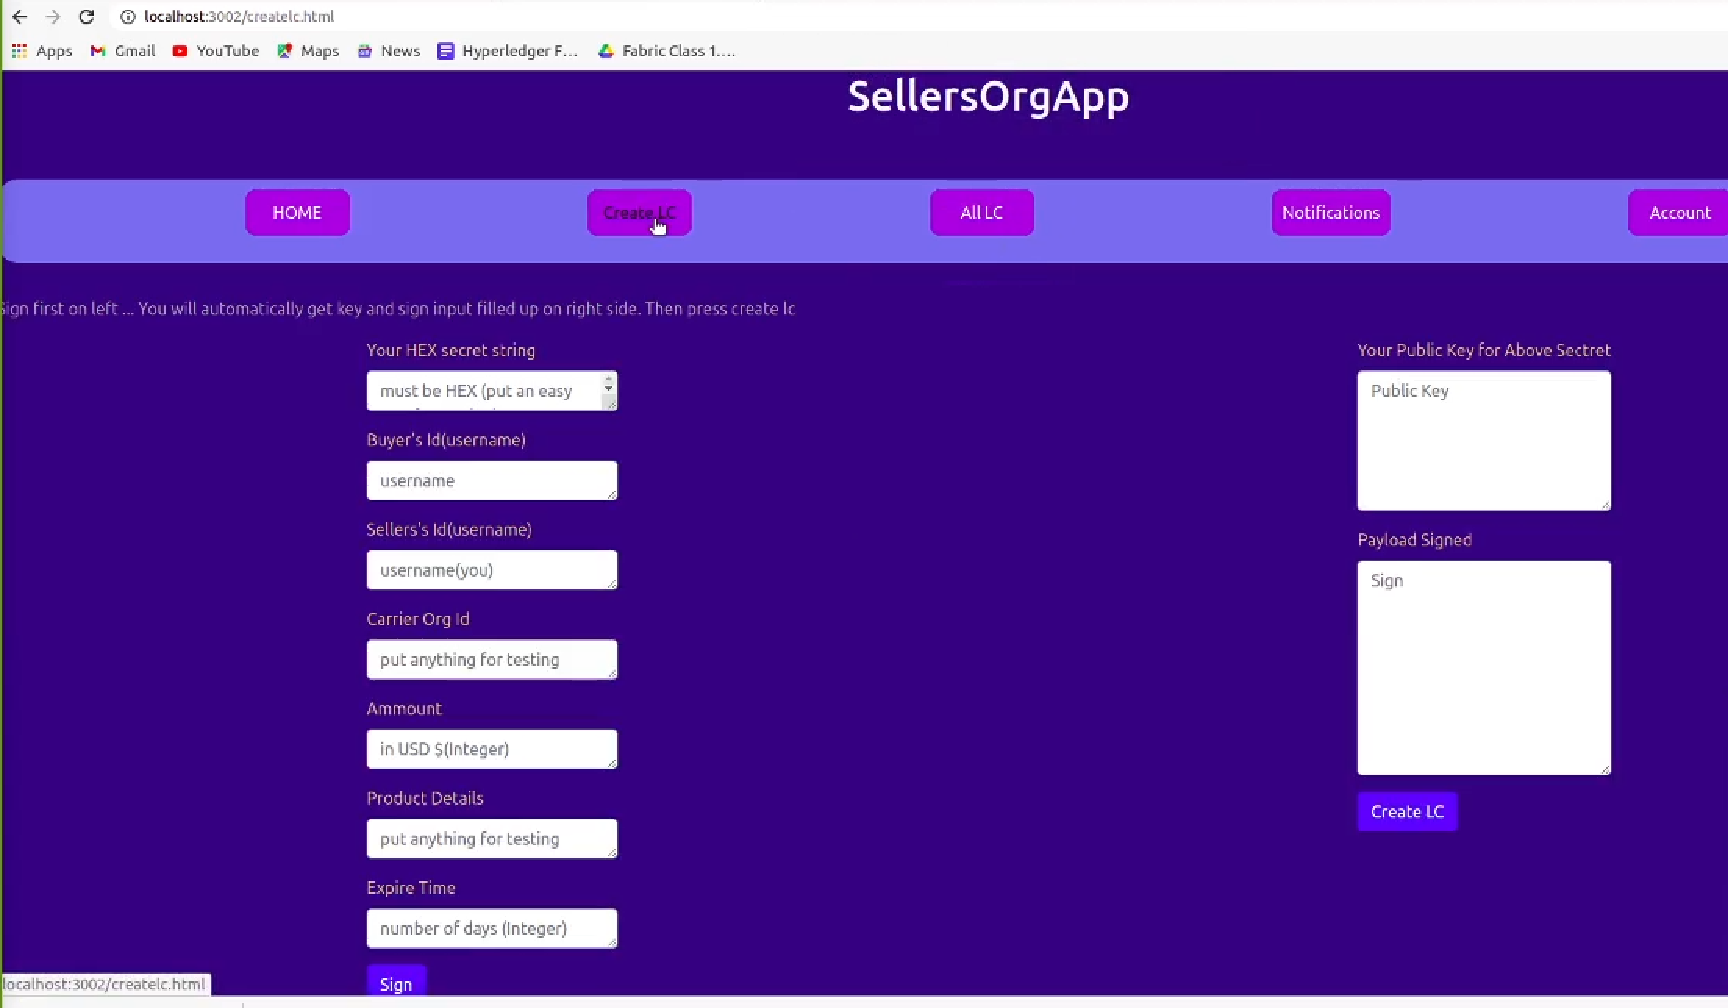
\includegraphics[width=0.7\paperwidth]{5.pdf}
    \caption{Seller siging}
    \label{fig:5}
\end{figure}

\begin{figure}[t]
    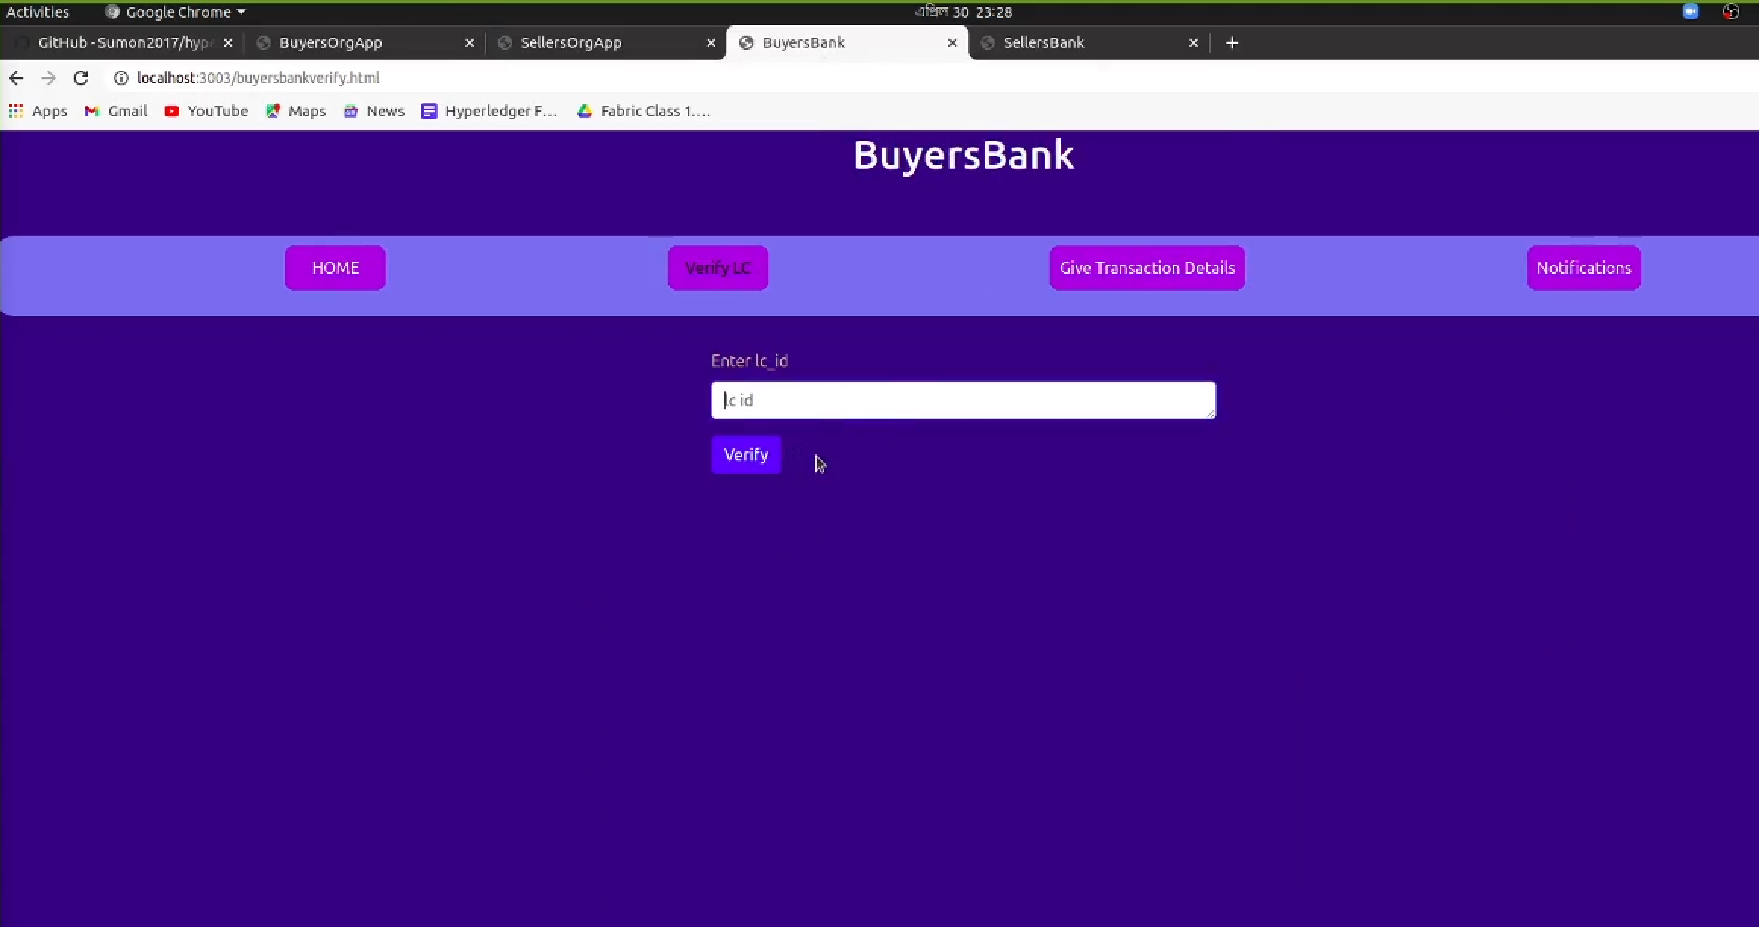
\includegraphics[width=0.7\paperwidth]{7.pdf}
    \caption{Buyers Bank Verifying}
    \label{fig:7}
\end{figure}


\begin{figure}[b]
    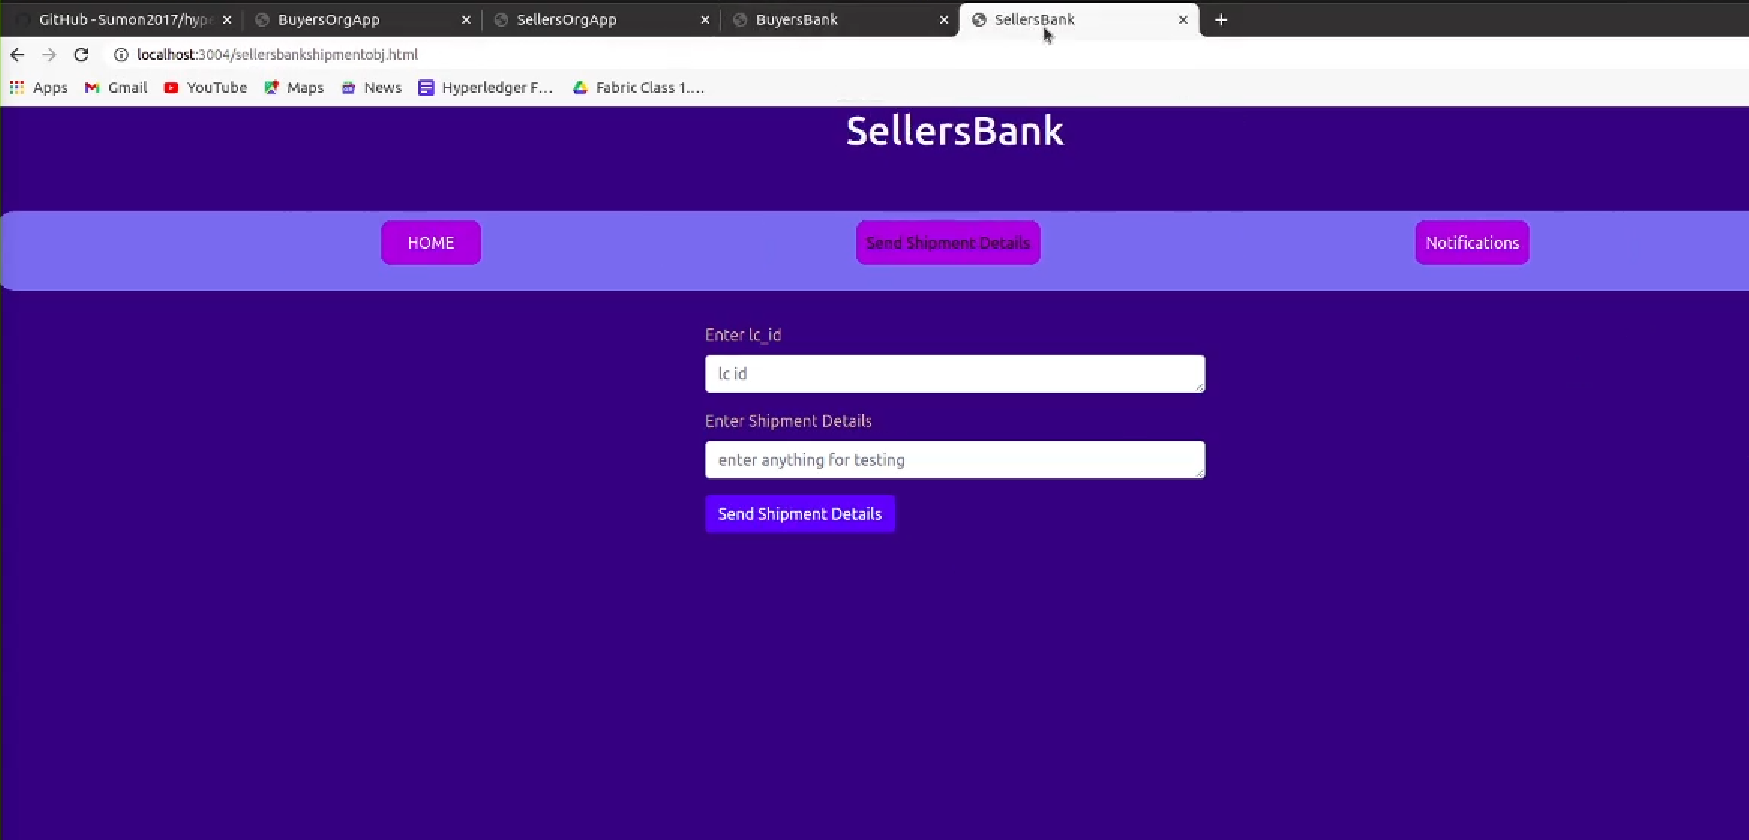
\includegraphics[width=0.7\paperwidth]{8.pdf}
    \caption{Sellers Bank sending shipment details}
    \label{fig:8}
\end{figure}


\chapter{Analysis}

In our project or system, following activities from different organization are done one by one maintaining these rules :
\begin{itemize}
\item At first, Seller initiates the LC.
\item Buyer approves LC pointed towards it, if everything is okay with the LC and sellers sign.
\item Then Buyers bank issues LC after checking both buyer and seller sign.
\item All sign verification is done inside the chaincode (not server).
\item Buyers can verify and sign only if the lc\_status is initial.
\item Buyers bank can verify and issue LC only if the lc\_status is approved.
\item Sellers bank can send shipment details only if the lc\_status is issued.
\item Buyers bank can send transaction details only if the lc\_status is shipped.
\item Everything should be under lc\_expire time.
\end{itemize}

We can say that the main users of project or system are Seller(Exporter), Buyer(Importer), SellerBank(Advising Bank), BuyerBank(Issuing Bank).

\vspace{20pt}
{\large Figure \ref{fig:analysis} shows the main activity of our project.}
\begin{figure}[h]
    \centering
    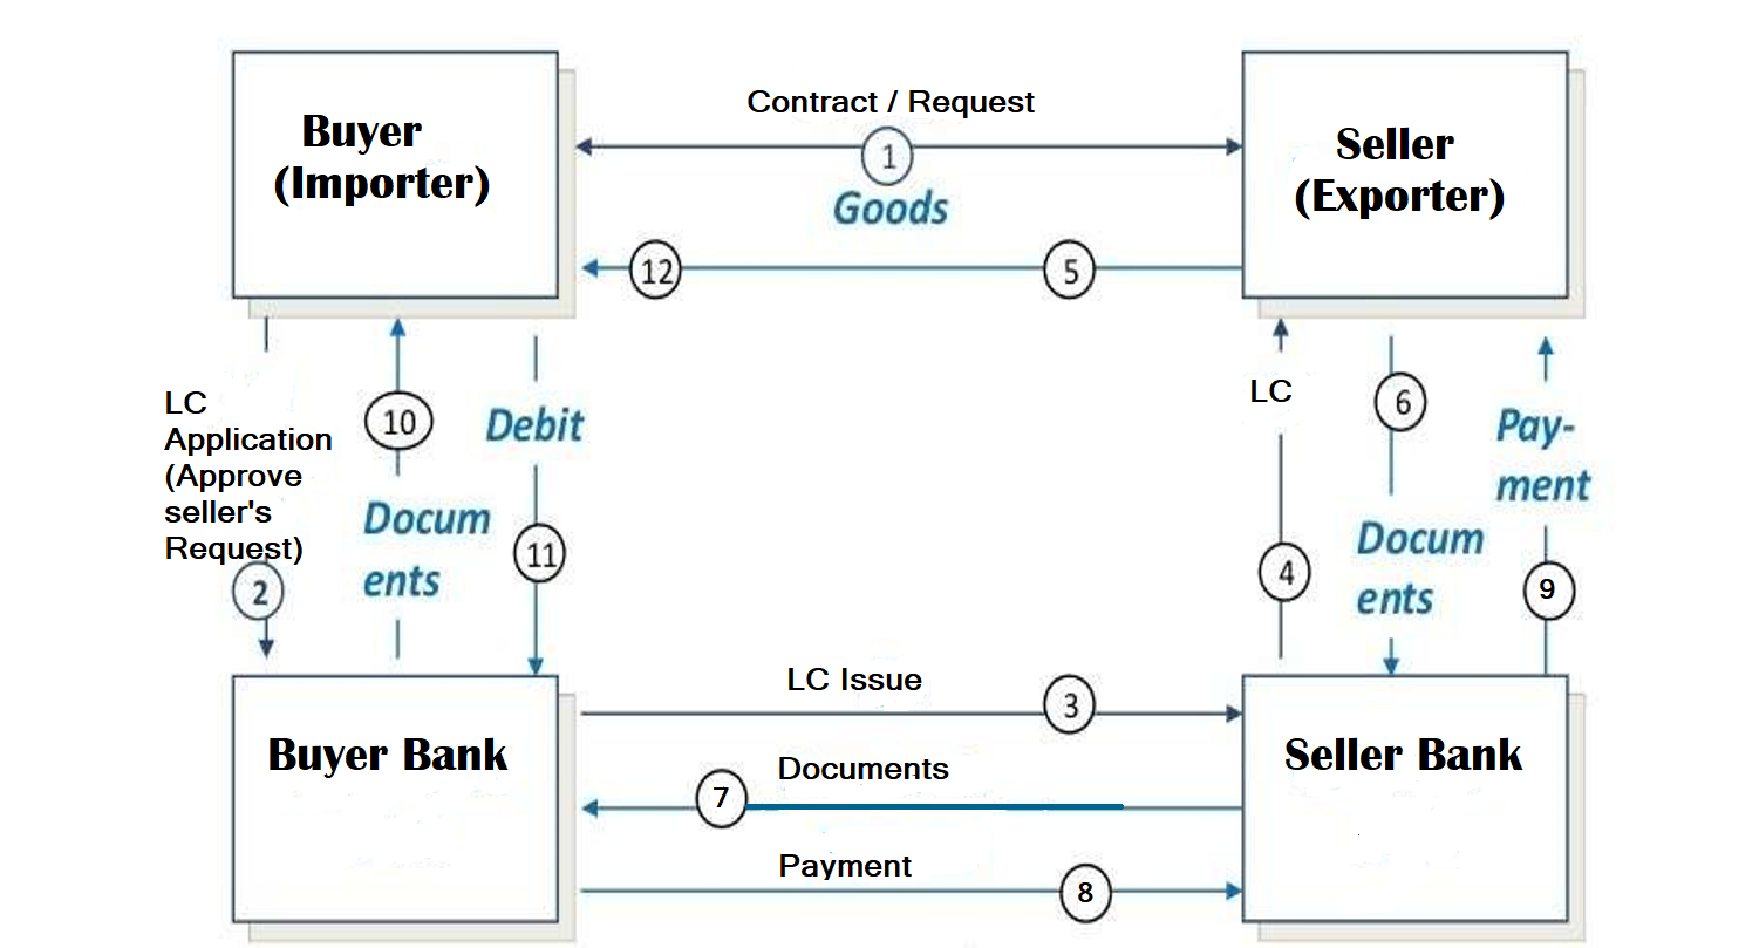
\includegraphics[width=1.1\textwidth]{Picture1.pdf}
    \caption{Overall Main Activity and its flow}
    \label{fig:analysis}
\end{figure}

\chapter{Conclusion}

In this project, The application of blockchain to Letter of Credit can help streamline the manual processing of import/export documentation, improve security by reducing errors, make companies' working capital more predictable and increase convenience for all parties through mobile interaction.

\vspace{10pt}
Here are some limitations of our project -
\begin{itemize}
    \item it is possible to create many seller and buyer member through sign up. But, for the simplicity, we have restricted only one Seller Bank and one Buyer Bank.
    
    \item The utility service can also be implemented in complex frontend app or users own  managed server. We haven't implemented such kind of utility services.
    
    \item We have created four organization app/browser's tab for four organizations. It can be wrapped up within only one app.
\end{itemize}


The project can be improved by further work on ``Invoice \& Legal Documents Management" , ``Well defined frontend utility service implementation", ``Ensuring Account, Stock price accuracy" etc.
\renewcommand{\bibname}{References}
\bibliographystyle{plain}
\bibliography{blockchain}


\end{document}
